\documentclass[11pt]{article}

\usepackage[T1]{fontenc}
\usepackage[english]{babel}
\usepackage[a4paper,margin=2.6cm]{geometry}
\usepackage{amsmath,amssymb,amsthm}
\usepackage[hidelinks]{hyperref}
\usepackage{amsthm}
\usepackage{subcaption}

% --- Notation ---
\newcommand{\N}{\mathbb{N}}
\newcommand{\minClases}{\operatorname{minClases}}
\newcommand{\chisemi}{\chi_{\mathrm{semi}}}


% Menos espacio entre figuras
\setlength{\floatsep}{8pt}        % entre figuras (floats)
\setlength{\textfloatsep}{8pt}    % entre figura y texto
\setlength{\intextsep}{8pt}       % figura "en el texto"


\theoremstyle{definition}
\newtheorem{definition}{Definition}[section]

\theoremstyle{plain}
\newtheorem{theorem}[definition]{Theorem}
\newtheorem{lemma}[definition]{Lemma}

\theoremstyle{remark}
\newtheorem{remark}[definition]{Remark}
% Figures (TikZ)
\usepackage{tikz}
\usetikzlibrary{calc,positioning,decorations.pathreplacing,arrows.meta,babel}



\title{Forbidden Colored Patterns on Triples:\\a Systematic Family of Graph Parameters}
\author{Germ\'an Javier Rud%
\thanks{B.Sc.\ in Business Administration (UADE). B.Sc.\ candidate in Data Science at the Faculty of Exact and Natural Sciences, University of Buenos Aires (final two courses).}%
\and Eric Brandwein%
\thanks{Thesis supervisor (B.Sc.\ in Data Science, University of Buenos Aires).}}
\date{\today}

\begin{document}
\maketitle

\begin{abstract}
This work builds on a B.Sc.\ thesis in Data Science at the University of Buenos Aires (Faculty of Exact and Natural Sciences),
supervised by Eric Brandwein, and continues in the current manuscript.

We study a systematic family of graph parameters defined via \emph{forbidden colored patterns} on ordered triples.
Given a small set of patterns on three positions, the parameter is the minimum number of parts in a vertex partition
(together with a vertex order) that avoids all patterns on every ordered triple.
This framework is inspired by the ``order + partition'' viewpoint behind thinness and its variants and provides a uniform way to
generalize graph classes and measure distance to them.
We analyze several families motivated by star-like, bipartite-like, and forest-like constraints, identify collapses to classical
invariants in multiple cases, and outline complexity and algorithmic directions suggested by the resulting landscape.
\end{abstract}

\section{Motivation: thinness, variants, and forbidden patterns}

Thinness is a width parameter that generalizes interval graphs: interval graphs are exactly the graphs of thinness~$1$,
and bounded thinness is used to extend algorithmic techniques beyond interval graphs \cite{Shitov2025}.
A common motivation in the thinness literature is that many problems that are hard in general
become polynomial-time solvable on graphs of bounded thinness, provided a suitable certificate
(order + partition) is available \cite{BB2021}.

Proper thinness is defined analogously, as an interval-like generalization of \emph{proper} interval graphs.
Conceptually, it strengthens thinness by adding a second consistency requirement (the reverse order),
which can be viewed as forbidding an additional local configuration (a ``reverse'' pattern) \cite{BB2021}.

\medskip
\noindent\textbf{Why go beyond interval graphs?}
Proper thinness can be seen as ``thinness + one more forbidden pattern'' (the reverse constraint).
This motivates a broader question: what happens if we take \emph{other} small collections of forbidden colored patterns
and define the minimum number of parts needed to avoid them?
If these parameters preserve useful properties of the underlying class they generalize,
then problems solvable efficiently on that class may remain solvable (or become parametrically tractable)
when the parameter is bounded.

\section{Framework: forbidden colored patterns}

The use of forbidden patterns on three vertices as class descriptors is inspired by the systematic study of
such classes in \cite{FeuilloleyHabib2018}.

\subsection{Patterns, solutions, avoidance}

\begin{definition}[Colored pattern on three positions]
A \emph{colored pattern} is a triple \(P=(A,N,C)\) where
\[
A,N \subseteq \binom{\{1,2,3\}}{2},
\qquad
C \in \binom{\{1,2,3\}}{2}.
\]
Elements of \(\binom{\{1,2,3\}}{2}=\{\{1,2\},\{1,3\},\{2,3\}\}\) are interpreted as pairs of \emph{positions}
in an ordered triple \((1\prec 2\prec 3)\).
The set \(A\) specifies edges that \emph{must} be present, \(N\) specifies edges that \emph{must not} be present,
and the pair \(C\) indicates which two positions are required to lie in the \emph{same} part of a partition.
\end{definition}

\begin{definition}[Solution and value]
Let \(G=(V,E)\). A \emph{solution} is a pair \(S=(\prec,\mathcal Q)\), where \(\prec\) is a total order on \(V\)
and \(\mathcal Q=\{V_1,\dots,V_k\}\) is a partition of \(V\).
The \emph{value} of \(S\) is \(|\mathcal Q|=k\).
\end{definition}

\begin{definition}[Avoiding a pattern]
Fix a graph \(G\) and a solution \(S=(\prec,\mathcal Q)\).
Given three distinct vertices \(x\prec y\prec z\) (written as \((v_1,v_2,v_3)=(x,y,z)\)),
we say \((x,y,z)\) \emph{avoids} \(P=(A,N,C)\) if at least one of the following holds:
\begin{enumerate}
\item some required edge from \(A\) is missing in \(G[\{x,y,z\}]\);
\item some forbidden edge from \(N\) is present in \(G[\{x,y,z\}]\);
\item the pair of positions \(C=\{i,j\}\) lands in different parts of \(\mathcal Q\).
\end{enumerate}
The solution \(S\) \emph{avoids} \(P\) if every triple \(x\prec y\prec z\) avoids \(P\).
For a finite family of patterns \(\mathcal P\), the solution avoids \(\mathcal P\) if it avoids each \(P\in\mathcal P\).
\end{definition}

\begin{definition}[Parameter induced by forbidden patterns]
For a finite family of patterns \(\mathcal P\), define
\[
\minClases_{\mathcal P}(G)
=
\min\{\,|\mathcal Q|:\ (\prec,\mathcal Q)\text{ is a solution for }G\text{ that avoids all }P\in\mathcal P\,\}.
\]
\end{definition}



% --- Figure: pattern ---
\begin{figure}[h]
\centering
\begin{tikzpicture}[
  font=\small,
  every node/.style={circle, draw, inner sep=1.4pt},
  >=latex
]
\node[draw=red, very thick, fill=red!12] (p1) at (0,0) {1};
\node (p2) at (1.7,0) {2};
\node[draw=red, very thick, fill=red!12] (p3) at (3.4,0) {3};

\draw[line width=0.6pt] (p1)--(p2);
\draw[densely dashed, line width=0.6pt] (p2)--(p3);

\node[draw=none] at (1.7,-0.95) {$A=\{\{1,2\}\}$,\ $N=\{\{2,3\}\}$,\ $C=\{1,3\}$};
\end{tikzpicture}
\caption{A forbidden colored pattern (solid = required, dashed = forbidden, red = same part).}
\label{fig:tiny-pattern}
\end{figure}



A certificate consists of a total order \(\prec\) on \(V(G)\) and a partition \(\mathcal Q\) of \(V(G)\) such that every ordered triple \(x\prec y\prec z\) avoids all forbidden patterns in \(\mathcal P\).
Equivalently, \(\minClases_{\mathcal P}(G)\) is the minimum number of parts in such a certificate.




\section{Why this generalizes graph classes}

If \(\minClases_{\mathcal P}(G)=1\), then the entire graph must avoid \(\mathcal P\), so \(G\) belongs to the class
defined by those forbidden patterns. This justifies viewing the parameter as a ``distance'' to the class:
larger values measure how many parts are needed so that each part (together with the same order) avoids the patterns.

This also parallels a familiar theme in width parameters. Treewidth and pathwidth generalize trees and paths by allowing
bounded-width decompositions; here, forbidden-pattern parameters generalize a target class by allowing a bounded number of
parts, each avoiding the same local obstructions.

\section{What we have been doing}

The research program is to analyze \emph{all} parameters obtained from combinations of forbidden colored patterns on
three positions. 

\begin{figure}[h]
\centering
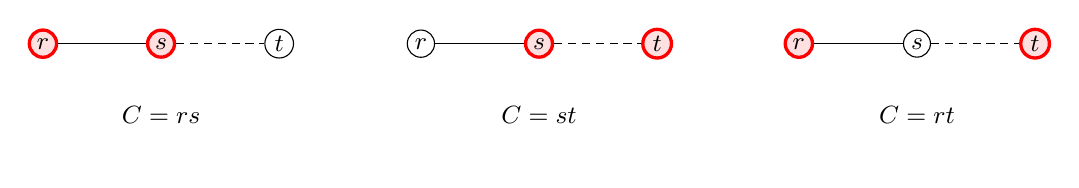
\begin{tikzpicture}[
  scale=1,
  every node/.style={circle, draw, inner sep=1.4pt, font=\small},
  same/.style={draw=red, very thick, fill=red!12},
  lab/.style={draw=none, font=\small},
  >=latex
]

% --- C = rs ---
\begin{scope}[shift={(0,0)}]
\node[same] (r) at (0,0) {$r$};
\node[same] (s) at (1.5,0) {$s$};
\node       (t) at (3,0) {$t$};
\draw (r)--(s);
\draw[densely dashed] (s)--(t);
\node[lab] at (1.5,-0.9) {$C=rs$};
\end{scope}

% --- C = st ---
\begin{scope}[shift={(4.8,0)}]
\node       (r) at (0,0) {$r$};
\node[same] (s) at (1.5,0) {$s$};
\node[same] (t) at (3,0) {$t$};
\draw (r)--(s);
\draw[densely dashed] (s)--(t);
\node[lab] at (1.5,-0.9) {$C=st$};
\end{scope}

% --- C = rt ---
\begin{scope}[shift={(9.6,0)}]
\node[same] (r) at (0,0) {$r$};
\node       (s) at (1.5,0) {$s$};
\node[same] (t) at (3,0) {$t$};
\draw (r)--(s);
\draw[densely dashed] (s)--(t);
\node[lab] at (1.5,-0.9) {$C=rt$};
\end{scope}

\end{tikzpicture}
\caption{Three basic ``colored'' constraints on the ordered positions \(r\prec s\prec t\), keeping fixed an \(\mathrm{est}\)-type edge template (solid \(rs\), dashed \(st\)).}
\label{fig:basic-C-examples}



\end{figure}



We denote by \(P_{rs}\), \(P_{st}\), and \(P_{rt}\) the full patterns obtained from the same edge template by choosing
\(C=\{r,s\}\), \(C=\{s,t\}\), and \(C=\{r,t\}\), respectively.
We write \(P_{rs\text{-}st}\) for the family \(\{P_{rs},P_{st}\}\), and similarly \(P_{rs\text{-}st\text{-}rt}\) for \(\{P_{rs},P_{st},P_{rt}\}\).
\medskip

\noindent
Beyond the three basic choices \(C\in\{rs,st,rt\}\) for a fixed edge template, we also study \emph{combinations of full patterns}.
That is, instead of imposing a single forbidden pattern \(P\), we impose a \emph{family} of forbidden patterns
\(\mathcal P=\{P^{(1)},P^{(2)},\dots\}\) and require solutions to avoid all of them simultaneously
(e.g., \(\mathcal P=\{P_{rs},P_{st}\}\), or \(\mathcal P=\{P_{rs},P_{st},P_{rt}\}\)).
\medskip


We started with families motivated by three familiar classes:
\begin{itemize}
\item \textbf{Star-like constraints:} many combinations collapse to vertex cover or chromatic number,
suggesting limited room for polynomial-time computability in general.
\item \textbf{Bipartite-like constraints:} some combinations admit clean exact formulas in terms of \(\chi(G)\).
\item \textbf{Forest-like constraints:} one combination matches vertex arboricity; several others do not match standard
parameters and appear structurally richer. We also studied variants ``given an order'' or ``given a partition''.
\end{itemize}



This systematic viewpoint is inspired by the classification of graph classes defined by forbidden patterns on three vertices in \cite{FeuilloleyHabib2018}.


\medskip

In the thesis manuscript, we focus on the star-based and bipartite-based families, while the forest-based family
is organized for a follow-up publication.

Finally, we note that a separate team is currently working on the parameter that generalizes path graphs.




\section{Future directions}

\begin{itemize}
\item \textbf{Continue the ``forest'' family.}
  We have analyzed the forest-based parameters up to the combinations
  \(\mathrm{for}_{rs,st}\) (in our current notation), and a natural next step is to
  complete the remaining cases in the same family. This includes:
  \begin{itemize}
  \item finishing the missing combinations and the corresponding class identifications (when they exist),
  \item completing the complexity landscape (polynomial-time cases vs.\ NP-hardness),
  \item and understanding the effect of fixing auxiliary information (e.g., ``given the order'' or ``given the partition'').
  \end{itemize}

\item \textbf{Compare with other graph parameters via domination.}
  A useful structural goal is to relate our parameters to established ones.
  If two parameters \(p\) and \(q\) satisfy
  \[
  p(G)\ \le\ f(q(G))
  \quad\text{for some computable function } f,
  \]
  then any algorithmic result that is efficient for bounded \(p\) can be transferred to bounded \(q\)
  (up to a loss captured by \(f\)). Conversely, if
  \[
  p(G)\ \ge\ g(q(G))
  \quad\text{for some computable function } g,
  \]
  then lower bounds or hardness results for bounded \(p\) can often be used to rule out
  analogous guarantees for bounded \(q\).
  We would like to systematically establish such relations with parameters such as
  treewidth/pathwidth, vertex arboricity, and coloring-based measures.

\item \textbf{Hybrid pattern families: generalizing two classes at once.}
  One promising direction is to combine patterns from different ``themes'' (e.g., a star-based constraint together
  with a forest-based constraint), creating parameters that simultaneously generalize two graph classes.
  For instance, mixing constraints of the form \(\mathrm{est}_1\) and \(\mathrm{for}_3\) produces a hybrid family.
  These hybrids may be structurally more constrained, which raises the question of whether some of them
  have a better chance of being computable in polynomial time (or admit stronger certificates).

\item \textbf{Algorithmic applications under bounded parameters.}
  Beyond identifying a parameter with a classical invariant, an important goal is to find concrete graph problems
  that become tractable when the parameter is bounded \emph{and} one can exploit the explicit certificate
  (order + partition) provided by a consistent solution.
  Two complementary perspectives are relevant:
  \begin{itemize}
  \item If a problem admits an efficient algorithm parameterized by an \(\mathrm{est}\)-type parameter by explicitly
    using the structure of a consistent solution (whether given as part of the input or constructed),
    this may either (a) imply new algorithmic consequences for coloring-type parameters, or (b) show that the
    \emph{certificate structure}, not just the numeric value, is algorithmically meaningful.
  \item Since the forest-generalizing parameters do not seem to collapse to standard measures in several cases,
    it is particularly worthwhile to search for problems that are tractable for these parameters but not known
    to be tractable under more classical ones. This would position such parameters as additional tools in the
    ``graph algorithm toolbox'' for practical instances.
  \end{itemize}

  In the language of parameterized complexity, the target is to obtain algorithms in:
  \begin{itemize}
  \item \textbf{FPT:} running time \(O(f(k)\,n^c)\), where \(k\) is the parameter, \(c\) is a constant, and \(f\) is
    an arbitrary computable function;
  \item \textbf{XP:} running time \(O(f(k)\,n^{g(k)})\), for computable functions \(f\) and \(g\).
  \end{itemize}
\end{itemize}
\section*{References (short, for the summary)}
\begin{thebibliography}{9}

\bibitem{BB2021}
F.~Bonomo and M.~Braberman.
\newblock \emph{Intersection models and forbidden pattern characterizations for 2-thin and proper 2-thin graphs}.
\newblock arXiv:2104.03937, 2021.

\bibitem{Shitov2025}
Y.~Shitov.
\newblock \emph{Graph thinness: a lower bound and complexity}.
\newblock Pacific Journal of Mathematics 339(2), 2025.

\bibitem{FeuilloleyHabib2018}
L.~Feuilloley and M.~Habib.
\newblock \emph{Graph classes and forbidden patterns on three vertices}.
\newblock arXiv:1812.05913, 2018.

\end{thebibliography}








\end{document}